%!TEX root = ../thesis.tex
%*******************************************************************************
%****************************** Second Chapter *********************************
%*******************************************************************************

\chapter{Parameter Estimation for Hidden Markov Models}~\label{chapter:parameter_estimation}

\ifpdf
    \graphicspath{{Chapter2/Figs/Raster/}{Chapter2/Figs/PDF/}{Chapter2/Figs/}}
\else
    \graphicspath{{Chapter2/Figs/Vector/}{Chapter2/Figs/}}
\fi

\section{Expectation–Maximization algorithm}~\label{sec:EM}
 
Also abbreviated as \textbf{EM algorithm} is an iterative approach for maximum likelihood estimates of model parameters. 
It is used in situations where incomplete data are present therefore a part of a complete data set is hidden, 
and we may not be able to apply straightforward analytical procedures for computing maximum likelihood estimates as in a 
case of complete data. EM algorithm introduce further below is mainly based on the work of \citep{Dempster1977} and \citep{McLachlan2008}.

In other words, we want to find the best estimate of the parameters for which the observed sequence of emissions is the most likely. 
This is of great importance and efficiency in Hidden Markov models where we have a space of emissions and states, where  emissions 
are observed and states are hidden. We also know that the state space is, in our case, finite, and therefore we can enumerate all possible states 
since the emissions are independent but not identically distributed, s.t.\ the distribution of emissions depends on the hidden state.

Let us also denote $\theta \in \Theta$ which is a vector of parameters belonging to parameter space $\Theta$. 
The aim of EM algorithm is essentially to find the "best" estimate of $\theta$ that maximizes the likelihood function $L(\theta|\textbf{Y})$, 
this is well known as Maximum likelihood estimate (MLE) that leads to the estimate $\hat{\theta}_{MLE}$. 

\subsection*{Complete data}

If we assume that the data are complete, i.e. we have a complete set of observations $\textbf{Y} = \{y_1,\ldots,y_T\}$, and we discard the hidden states, 
then MLE results in the following optimization problem: 

\begin{equation}
    \hat{\theta}_{MLE} = \underset{\theta \in \Theta}{\arg\max} L(\theta|\textbf{Y}) = \underset{\theta \in \Theta}{\arg\max} \prod_{t=1}^{T} f(y_t|\theta)
\end{equation}

where $f(y_t|\theta)$ is a probability density function of a random variable $Y_t$ given a parameter $\theta$.

To apply the approach for complete data, let us consider daily log-returns of BTC/USDT trading pair in past 5 years. 
Plotting the histogram we conclude that the log-returns may asymptotically follow normal distribution. 
Since the probability density function in such case is unimodal and has only one global maximum, 
the logarithmic transformation of likelihood function conveniently converts multiplication to addition with the 
preservation of global maximum to be optimized by taking the partial derivative w.r.t.\ each parameter. 
First, we formulate the likelihood function of two-parametric normal distribution $\mathcal{N}(\mu,\sigma^2)$ given an observed sequence 
of log-returns $\textbf{Y} = \{y_1,\ldots,y_T\}$ where $T \in \mathbb{N}$:
 
\begin{equation}
    L(\mu,\sigma^2|\textbf{Y}) = \prod_{t=1}^{T} \frac{1}{\sqrt{2\pi \sigma^2}} e^{-\frac{1}{2} \frac{{(y_t-\mu)}^2}{\sigma^2}}
\end{equation}

\begin{equation}
    \ell(\mu,\sigma^2|\textbf{Y}) = \sum_{t=1}^{T} \ln L(\mu,\sigma^2|y_t) 
\end{equation}

where $x_1,\ldots,x_N$ is a vector of log-returns of length N and $\mu$ and $\sigma^2$ are parameters to be estimated. 

\begin{equation}
    \ell(\mu,\sigma^2|\textbf{Y}) = -\frac{T}{2} \ln(2 \pi) - \frac{T}{2} \ln(\sigma^2) - \frac{1}{2 \sigma^2} \sum_{t=1}^{T} {(y_t - \mu)}^2
\end{equation}

If we now take the partial derivative w.r.t.\ the parameter $\mu$ and $\sigma^2$ and set it to zero we obtain the ML estimate of the 
parameters as follows:

\begin{gather} 
\frac{\partial \ell(\mu,\sigma^2|\textbf{Y})}{\partial \mu}  = \frac{1}{\sigma^2} (\sum_{t=1}^{T} y_t - T\mu) \nonumber \\
0 = \frac{1}{\sigma^2} (\sum_{t=1}^{T} y_t - T\mu) \nonumber\\
\hat{\mu}_{MLE} = \frac{\sum_{t=1}^{T} y_t}{T} \label{eq:MLEmu}
\end{gather}

\begin{gather} 
\frac{\partial \ell(\mu,\sigma^2|\textbf{Y})}{\partial \sigma^2}  = -\frac{T}{\sigma}+ \frac{1}{\sigma^3} \sum_{t=1}^{T} {(y_t - \mu)}^2 \nonumber\\
0 = -\frac{T}{\sigma}+ \frac{1}{\sigma^3} \sum_{t=1}^{T} {(y_t - \mu)}^2 \nonumber\\
\hat{\sigma}_{MLE}^2 = \frac{\sum_{t=1}^{T} {(y_t - \mu)}^2}{T} \label{eq:MLEsigma} 
\end{gather}

\subsection*{Incomplete data}

Although the assumption of complete data simplifies the analytical procedure of calculating the ML estimate in closed form, 
it is not applicable for incomplete data, i.e. when certain information is latent. This is particularly applicable for Hidden Markov Models. 
The alternative for the likelihood function of the complete data is therefore to use a joint probability of observed and hidden part of the data to 
obtain a marginal probability by summing over all possible hidden states $i \in I$, as per \citep{Jurafsky2008} and \citep{Devavrat2014}:

\begin{align} \label{eq:loglike}
\ell(\theta|\textbf{Y}) = \sum_{t=1}^{T} \ln \mathbb{P}(Y_t= y_t|\theta) & = \sum_{t=1}^{T} \ln \sum\limits_{i=1}^N \mathbb{P}(Y_t= y_t,X_t=i|\theta) \\
 & = \sum_{t=1}^{T} \ln \sum\limits_{i=1}^N \mathbb{P}(Y_t= y_t|X_t=i,\theta) \mathbb{P}(X_t=i|\theta) \nonumber \\
\end{align}

Since the natural logarithm is strictly monotonic increasing function the value of $\theta$ maximizes the log-likelihood as well as the 
likelihood function. Simply, the EM algorithm iterates over possible values of $\theta$ to find the best estimate in terms of log-likelihood difference, 
i.e.\ until convergence criterion, in \citep{McLachlan2008}, is satisfied:

\begin{equation} \label{eq:conv}
|\ell(\theta^{(k)}|\textbf{Y}) - \ell(\theta^{(k-1)}|\textbf{Y})| \leq \epsilon 
\end{equation}

where the current estimate of $\theta$ for k-th iteration is denoted with superscript $(k)$ 
and the convergence threshold $\epsilon$. 

Since the log-likelihood function in Equation \ref{eq:loglike} is not analytically tractable, according to \citep{Bishop2006}, and involves logarithm of a sum,
we need to find an alternative approach to estimate the parameters.
It is, however, possible to introduce several assumptions that will eventually suffice in providing 
direct iterative solution to the optimization problem. Let us first construct a lower bound for the 
marginal likelihood in Equation \ref{eq:loglike}.

We introduce density function $q(x)$ called "averaging distribution" and start by multiplying 
the joint likelihood by $\frac{q(x)}{q(x)}$. Such expression will allow for a construction of 
artificial weights and with the use of Jensen's inequality, as suggested by \citep{Gu2008}:

\begin{align}
    \sum_{t=1}^{T} \ln \sum_{i=1}^{N} q(X_t = i) \frac{p(Y_t=y_t, X_t = i|\theta)}{q(X_t = i)} \geq& \sum_{t=1}^{T} \sum_{i=1}^{N} q(X_t = i) \ln \frac{p(Y_T =y_t, X_t = i|\theta)}{q(X_t = i)} \\
    \ell(\theta|\textbf{Y}) \geq& L(\theta,q|\textbf{Y}), \quad \forall q \in Q
\end{align}

where $Q$ is a set of all possible probability distributions.

The constructed lower bound $L(\theta,q|\textbf{Y})$ can be factorized into the expectation 
of the joint log-likelihood w.r.t to distribution $q(x)$ and entropy $H(q)$:

\begin{equation}
    L(\theta,q|\textbf{Y}) = E_{q(x)} [\ln p(\textbf{X},\textbf{Y}|\theta)] + H(q)
\end{equation}

where $E_{q(x)} [\ln p(X,Y|\theta)]$ is called the \textbf{expectation of complete data log-likelihood function} (or Q-function).
Moreover, $H(q)$ is a constant and does not depend on the parameter $\theta$ and therefore can be omitted from the
optimization problem. Therefore, decoupling the log-likelihood function into two parts, we obtain the following expression:

\begin{equation}
    \ell(\theta|\textbf{Y}) = E_{q(x)} [\ln p(\textbf{X},\textbf{Y}|\theta)] + D_{KL} (q(\textbf{X}) || p(\textbf{X}| \textbf{Y},\theta))
\end{equation}

where $D_{KL}$ is the \textit{Kullback-Leibler divergence} between the distribution $q(x)$ and the posterior distribution $p(\textbf{X}|\textbf{Y},\theta)$.
The Kullback-Leibler divergence is a measure of dissimilarity between two probability distributions, and we may interpret it as a geometrical statistical distance.
It is also asymmetric and non-negative, and it is zero if and only if the two probability measures are equal which is a result of \textit{Gibb's inequality}. \citep{Csiszar1975}
These properties are of great importance in the EM algorithm because in order to minimize the distance between the two distributions as described above,
\citep{Bishop2006} states to set the distribution $q(x)$ equal to the posterior distribution $p(\textbf{X}|\textbf{Y},\theta)$.

This, first step of the algorithm abbreviated as \textbf{E-step} results in estimating the function $q$ for a $\theta^{k}$, given the k-th iteration of EM algorithm, 
that maximizes the lower bound $L(\theta,q|\textbf{Y})$. s.t. the "distance" from the lower bound to log-likelihood function $\ell(\theta|\textbf{Y})$ is minimized:

\begin{equation} \label{eq:qnew}
    q^{(k+1)} = \underset{q \in Q}{\arg\max} L(\theta^{(k)},q|\textbf{Y}) = p(\textbf{X}|\textbf{Y},\theta^{(k)})
\end{equation}

In other words, we want to minimize distance between the complete data log-likelihood function $L(\theta,q|\textbf{Y})$ and incomplete data $\ell(\theta|\textbf{Y})$ 
with respect to function $q(x)$. Kullback-Leibler divergence (hereafter KL divergence) measure is commonly used in image or signal processing 
in calculation of the expected excess surprise from using $q$ as a probability distribution for our model given that the true or actual 
probability distribution is $p$. \citep{Balesdent2016} 

Substantially, the measure is a difference of cross-entropy denoted by $H(p,q)$ and entropy by $H(p)$ which is also always non-negative as a result of Gibb's inequality.

\begin{align}
    D_{KL} (p || q) & = \sum_{X} p(x) \ln \frac{p(x)}{q(x)} \\
                    & = \sum_{x} p(x) \ln \frac{1}{q(x)} - \sum_{x} p(x) \ln \frac{1}{p(x)} \\
                    & = H(p,q) - H(p)
\end{align}

More rigorously, we have only defined the lower bound for the complete data log-likelihood function using arbitrary probability function $q(x)$, 
but the deeper examination of the lower bound with the use of KL divergence directly yields the choice of marginal posterior 
distribution $p(\textbf{X}|\textbf{Y},\theta)$ for the probability function $q(x)$:

\begin{align}
    L(\theta,q|\textbf{Y}) &= \sum_{i=1}^{N} q(X = i) \ln \frac{p(X = i,\textbf{Y}|\theta)}{q(X = i)} \\
    & = \sum_{i=1}^{N} q(X = i) \ln \frac{p(X = i|\textbf{Y},\theta) p(\textbf{Y}| \theta)}{q(X = i)} \\
    & = \sum_{i=1}^{N} q(X = i) \ln p(\textbf{Y}|\theta) + \sum_{i=1}^{N} q(X = i) \ln \frac{p(X = i|\textbf{Y},\theta)}{q(X = i)} \\
    & =  \ell(\theta|\textbf{Y}) - D_{KL}(q(\textbf{X})||p(\textbf{X}|\textbf{Y},\theta))
\end{align}

Now we see that the statistical distance between the two likelihood functions is determined solely by the KL divergence. Similarly, it can be shown that Equation \ref{eq:qnew} is a 
minimization problem of KL divergence between the two distributions $q$ and $p$:

\begin{equation}
    q^{(k+1)} = \underset{q \in Q}{\arg\min}(\ell(\theta|\textbf{Y}) - L(\theta, q|\textbf{Y})) = \underset{q \in Q}{\arg\min}  D_{KL} (q(\textbf{X}) || p(\textbf{X}| \textbf{Y},\theta^{(k)}))
\end{equation}

To visualize the EM algorithm, refer to Figure \ref{fig:Loglike} where red curve is the log-likelihood function $\ell(\theta|\textbf{Y})$
and notice that the blue curve already represents the lower bound
after the first iteration of E-step yielding $q^{(k)}$ as a solution. Afterwards parameter estimates of $\theta^{(k)}$ are obtained as part of the M-step 
s.t. the next iteration of E-step can be performed, and the lower bound is maximized again represented by the green curve.

Until now, we have considered the optimal manner in which we compute the conditional expectation $E_{\textbf{X}|\textbf{Y},\theta^{(k)}} [\ell(\theta|\textbf{Y})]$ by 
finding the appropriate function $q$. Next step is, as typical for coordinate descent, selection of parameter $\theta^{(k+1)}$, 
with already estimated $q^{(k+1)}$, that maximizes the lower bound $L(\theta,q|\textbf{Y})$. The goal of M-step is according to \citep{Dempster1977} and \citep{Gu2008}:

\begin{equation}
    \theta^{(k+1)} = \underset{\theta \in \Theta}{\arg\max} L(\theta, q^{(k+1)}|\textbf{Y})
\end{equation}

\begin{figure}[ht]

    \begin{center}
        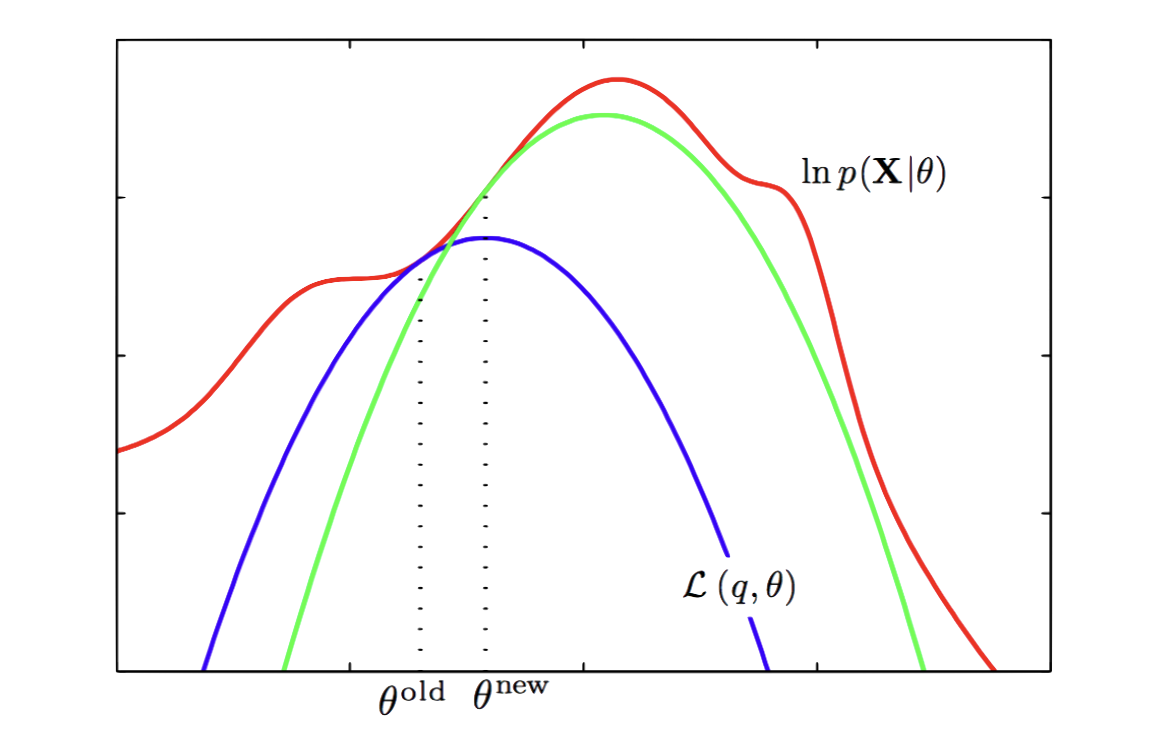
\includegraphics[width=0.9\textwidth]{Figs/Loglike.png}
    \end{center}

    \caption[Construction of log-likelihood lower bound in EM algorithm]{\textit{E-step as a problem of minimization of KL divergence represented as a gap between two likelihood functions followed by new estimate of $\theta$ within M-step, reprinted from \citep{Bishop2006}}}
    \label{fig:Loglike}
\end{figure}

\noindent Thus, as a summarization, the EM algorithm involves two steps:

\begin{itemize}
\item[1)] \textbf{Expectation step (E-step)} - choose a function q, i.e.\ probability distribution, that maximizes $L(\theta, q|\textbf{Y})$, which may be also viewed as 
                                               computing the posterior distribution $p(\textbf{X}|\textbf{Y},\theta^{(k)})$ based on $\theta^{(k)}$:

\begin{equation}
    Q(\theta|\theta^{(k)}) = E_{\textbf{X}|\textbf{Y},\theta^{(k)}} [\ell(\theta|\textbf{Y})]
\end{equation}

\item[2)] \textbf{Maximization step (M-step)} - estimate the parameter $\theta$ that maximizes the conditional expectation $E_{\textbf{X}|\textbf{Y},\theta^{(k)}} [\ell(\theta|\textbf{Y})]$.

\begin{equation}
    \hat{\theta}^{(k+1)} = \underset{\theta \in \Theta}{\arg\max} Q(\theta|\theta^{(k)}) 
\end{equation}

\end{itemize}

Both of these steps are repeated until convergence criterion given by Equation \ref{eq:conv} is attained assuming fixed tolerance $\epsilon$.

There is also generalized version of EM algorithm called \textbf{Generalized EM} (GEM) algorithm that allows for a more flexible approach
in the sense that it does not require the lower bound to be maximized in each iteration of E-step. Instead, at each iteration
the expected log-likelihood is increased by a certain amount but not locally maximized, i.e. is a form of gradient ascent. Such approach 
is particularly useful in cases where the lower bound is not analytically tractable, or the maximization problem is computationally infeasible, e.g. in case of cHMM with 
parametrized covariance matrix. However, it is important to note that the GEM algorithm does not guarantee convergence to a local maximum 
of the log-likelihood function and might converge after fewer iterations yielding a worse estimate of the parameters. \citep{Bishop2006} 

\subsection{Forward and Backward algorithm}

While given a sequence of emissions denoted by $\textbf{Y}, = \{y_0,y_1,\ldots,y_T\}$ and a model parameter vector $\theta = (\textbf{A},\textbf{B},\textbf{p})$, 
we need to express the likelihood function under the model constraints as follows:

\begin{align} \label{eq:loglikeFB}
    \mathcal{L}( \theta| \textbf{Y}) & = \prod\limits_{t=0}^T \sum\limits_{i=1}^N  \mathbb{P}(Y_t = y_t, X_t = i| \theta) \\
                                     & = \prod\limits_{t=0}^T \sum\limits_{i=1}^N  \mathbb{P}(Y_t = y_t | X_t = i, \theta) \mathbb{P}(X_t=i|\theta)
\end{align}

where $N$ denotes a number of hidden states. As in the previous chapter, we need to rather work with log-likelihood function which is more analytically convenient 
and allows us to avoid numerical underflow, as in Equation \ref{eq:loglike}, where summation is nested inside the logarithm, and therefore we cannot simply swap the order of summation and logarithm. Therefore, we need to find a way to compute the log-likelihood function 
in a more efficient way. Our goal is to estimate the posterior distribution of the hidden states given the observed sequence of emissions $p(\textbf{X}|\textbf{Y},\theta)$
that helps us to compute the expectation of the complete data log-likelihood function.

The summation in Equation \ref{eq:loglike} refers to all possible permutations of the sequence of hidden states \textbf{X} 
which implies that we would have $N^T$ possible sequences as seen in Figure \ref{fig:trellis}. Furthermore, in order to calculate $\mathcal{L}( \theta| \textbf{Y})$ we have $2TN^T$ 
operations which is also exponential in T and not feasible for real application. As opposed to brute-force infeasible
computation described above, we take a use of \textbf{Forward} and \textbf{Backward} pass to address \textbf{E-step} of the EM algorithm, as shown by \citep{Bishop2006} and \citep{Rabiner1989}.
Resulting algorithm requires time complexity of $O(TN^2)$\footnote{The O(n) symbol represents Big O notation, 
a convention in computer science to describe how an algorithm's running time or space needs grow as the input size increases. 
O(n) indicates that the growth is linear in relation to the input size n. \citep{Mohr2014}} 
for classical HMM and $O(TN(D+N))$ for HSMM which is a significant improvement. 

\begin{figure}[htbp]
    \begin{center}
    \begin{tikzpicture}[]
    % 1st column
    \node               at (0,6) {$t=0$};
    \node[state] (s1_1) at (0,5) {$S_1$};
    \node[mainstate] (s2_1) at (0,3.5) {$S_2$};
    \node[state] (s3_1) at (0,2) {$\ldots$};
    \node[state] (s4_1) at (0,0.5) {$S_N$};
    \node at (0,-0.5) {$y_0$};    % 2nd column
    \node               at (2,6) {$t=1$};
    \node[mainstate] (s1_2) at (2,5) {$S_1$}
        edge[lightedge] (s1_1)
        edge[lightedge] (s2_1)
        edge[lightedge] (s3_1)
        edge[lightedge] (s4_1);
    \node[state] (s2_2) at (2,3.5) {$S_2$}
        edge[lightedge] (s1_1)
        edge[lightedge] (s2_1)
        edge[lightedge] (s3_1)
        edge[lightedge] (s4_1);
    \node[state] (s3_2) at (2,2) {$\ldots$}
        edge[lightedge] (s1_1)
        edge[lightedge] (s2_1)
        edge[lightedge] (s3_1)
        edge[lightedge] (s4_1);
    \node[state] (s4_2) at (2,0.5) {$S_N$}
        edge[lightedge] (s1_1)
        edge[lightedge] (s2_1)
        edge[lightedge] (s3_1)
        edge[lightedge] (s4_1);
    \node at (2,-0.5) {$y_1$};
    % 3rd column
    \node               at (4,6) {$t=2$};
    \node[mainstate] (s1_3) at (4,5) {$S_1$}
        edge[lightedge]  (s1_2)
        edge[lightedge] (s2_2)
        edge[lightedge] (s3_2)
        edge[lightedge] (s4_2);
    \node[state] (s2_3) at (4,3.5) {$S_2$}
        edge[lightedge] (s1_2)
        edge[lightedge] (s2_2)
        edge[lightedge] (s3_2)
        edge[lightedge] (s4_2);
    \node[state] (s3_3) at (4,2) {$\ldots$}
        edge[lightedge] (s1_2)
        edge[lightedge] (s2_2)
        edge[lightedge] (s3_2)
        edge[lightedge] (s4_2);
    \node[state] (s4_3) at (4,0.5) {$S_N$}
        edge[lightedge] (s1_2)
        edge[lightedge] (s2_2)
        edge[lightedge] (s3_2)
        edge[lightedge] (s4_2);
    \node at (4,-0.5) {$y_2$};
    % 4th column
    \node               at (6,6) {$t=3$};
    \node[mainstate] (s1_4) at (6,5) {$S_1$}
        edge[lightedge]  (s1_3)
        edge[lightedge] (s2_3)
        edge[lightedge] (s3_3)
        edge[lightedge] (s4_3);
    \node[state] (s2_4) at (6,3.5) {$S_2$}
        edge[lightedge] (s1_3)
        edge[lightedge] (s2_3)
        edge[lightedge] (s3_3)
        edge[lightedge] (s4_3);
    \node[state] (s3_4) at (6,2) {$\ldots$}
        edge[lightedge] (s1_3)
        edge[lightedge] (s2_3)
        edge[lightedge] (s3_3)
        edge[lightedge] (s4_3);
    \node[state] (s4_4) at (6,0.5) {$S_N$}
        edge[lightedge] (s1_3)
        edge[lightedge] (s2_3)
        edge[lightedge] (s3_3)
        edge[lightedge] (s4_3);
    \node at (6,-0.5) {$y_3$};
    % 5th column
    \node               at (8,6) {$t=5$};
    \node[mainstate] (s1_5) at (8,5) {$S_1$}
        edge[lightedge]  (s1_4)
        edge[lightedge] (s2_4)
        edge[lightedge] (s3_4)
        edge[lightedge] (s4_4);
    \node[state] (s2_5) at (8,3.5) {$S_2$}
        edge[lightedge] (s1_4)
        edge[lightedge] (s2_4)
        edge[lightedge] (s3_4)
        edge[lightedge] (s4_4);
    \node[state] (s3_5) at (8,2) {$\ldots$}
        edge[lightedge] (s1_4)
        edge[lightedge] (s2_4)
        edge[lightedge] (s3_4)
        edge[lightedge] (s4_4);
    \node[state] (s4_5) at (8,0.5) {$S_N$}
        edge[lightedge] (s1_4)
        edge[lightedge] (s2_4)
        edge[lightedge] (s3_4)
        edge[lightedge] (s4_4);
    \node at (8,-0.5) {$y_4$};
    \end{tikzpicture}
    \end{center}
    \caption[Trellis as a result of Forward-Backward algorithm]{Trellis of the emission sequence $\{y_0,\ldots, y_4\}$ for T=4. Each node represents a state $S_i$ and each arc represents a transition from one state to another. The number of possible paths is $N^T$. }
    \label{fig:trellis}
    \end{figure}

\subsubsection*{Forward algorithm}

Each sequence can be decomposed into multiple subsequences which are shared among different sequences and do not need to be recomputed again. 
These subsequences can be represented by a trellis as shown in Figure \ref{fig:trellis}. With a help of such diagram we may imagine recording the probability of 
distinct subsequences at each time step $t$. In other words, we wish to compute a joint probability while taking advantage 
of the conditional independence of $Y_t$ given $X_t$ with respect to the remaining elements of the emission sequence that happen after time $t$. 
Moreover, due to Markov memoryless property, $X_t$ depends only on $X_{t-1}$. Let us now define the forward probability variable $\alpha_t(i)$ as in \citep{Bishop2006} and \citep{Rabiner1989}:

\begin{equation}
    \alpha_t(i) = \mathbb{P}(Y_t = y_t, Y_{t-1} = y_{t-1},\ldots, Y_0 = y_0 , X_t = i| \theta)
\end{equation}

Which we may also define as the probability of being in state i at time t after having observed the sequence $\{y_0,x_1,\ldots,y_t\}$. 
The calculation therefore results in recursively summing the incoming arcs at trellis nodes:

\begin{align} \label{eq: forward}
    \alpha_t(i) &= \mathbb{P}(Y_t = y_t, Y_{t-1} = y_{t-1},\ldots, Y_0 = y_0 , X_t = i| \theta) \\ \nonumber
                &= \mathbb{P}(Y_t = y_t | X_t = i, \theta) \mathbb{P}(Y_{t-1} = y_{t-1},\ldots, Y_0 = y_0 , X_t = i| \theta)  \\ \nonumber
                &= \mathbb{P}(Y_t = y_t | X_t = i, \theta) \sum\limits_{j = 1}^N \mathbb{P}(X_t = i| X_{t-1}=j,\theta) \alpha_{t-1}(j)\\ \nonumber
                &= b_i(y_t) \sum\limits_{j=1}^N a_{ji} \alpha_{t-1}(j)
\end{align}

In case the underlying hidden stochastic process is not strictly Markov but semi-Markov, the forward algorithm given by Equation \ref{eq: forward} is no longer valid since it assumes 
that the transitions are geometrically distributed. Let us use derivation from \citep{Yu2013} and \citep{Narimatsu2017}, and estimate parameters of a process that stays in state $i$ until time $t+d-1$ and then transits to another state $j$ at $t+d$. 
In order to account for the fact that the transitions are not geometrically distributed, we need to modify the forward variable $\alpha_t(i)$
s.t. the duration of the state follows some sojourn time distribution:

\begin{equation}
    \alpha_t(i,u) = \mathbb{P}(Y_t = y_t, Y_{t-1} = y_{t-1},\ldots, Y_0 = y_0 , X_t = i, \tau_t = u| \theta)
\end{equation}

Forward step in the algorithm can be defined in three steps:

\begin{itemize}
    \item[1.] \textbf{Initialization step}: For each $i \in I$ set value at time $t=0$ to:
    
    \begin{equation}
        \alpha_0(i)= p_i b_i(y_0)
    \end{equation}

    In case of semi-Markov process, we need to account for the sojourn time distribution $d_i(u)$ of the state $i$ at time $u$:

    \begin{equation}
        \alpha_0(i,u) = p_i b_i(y_0) d_i(u)
    \end{equation}

    \item[2.] \textbf{Induction step}: 
    
    \begin{equation}
        \alpha_t(i) = b_i(y_t) \sum\limits_{j=1}^N a_{ji} \alpha_{t-1}(j)
    \end{equation}

    Again, in case of semi-Markov process, we have the following recursive relationship, as proposed by \citep{Yu2013}, that holds for all $u \geq 1$:

    \begin{equation}
        \alpha_t(i,u) = \alpha_{t-1}(i,u+1) b_i(y_t) + \left( \sum\limits_{j \neq i} \alpha_{t-1}(j,1) a_{j,i} \right) b_i(y_t) d_i(u)
    \end{equation}

    where $d_i(u)$ is the duration of the state $i$ at time $u$ which is referred to as the sojourn time. 
    
    Afterwards, we recursively update current time index t to t+1 as long as $t \leq T$ starting at $t=1$.
    
    \item[3.] \textbf{Termination step}: once the iterative procedure is exhausted, i.e.\ when t=T we have the estimate of marginal likelihood of the observed sequence $\textbf{Y}$ under the model $\theta$ denoted as
    $\mathcal{L}(\theta| \textbf{Y})$:
    
    \begin{equation} \label{eq:loglikeF}
        \mathcal{L}(\theta| \textbf{Y}) = \sum_{i=1}^N \alpha_T(i)
    \end{equation}
    
    \end{itemize}

\subsubsection*{Backward algorithm}

While computing the backward probability variable denoted as $\beta_t(i)$ we assume the reversed iterative procedure. 
Let us define the backward probability $\beta$ variable as:

\begin{align} \label{eq: backward}
\beta_t(i)  &= \mathbb{P}(Y_{t+1} = y_{t+1}, Y_{t+2} = y_{t+2},\ldots, Y_T = y_T| X_t = i, \theta) \\ \nonumber
            &= \sum_{i,j}^N \mathbb{P}(Y_{t+1} = y_{t+1}, Y_{t+2} = y_{t+2},\ldots, Y_T = y_T,X_{t+1} = j | X_t = i, \theta)  \\ \nonumber
            &= \sum_{i,j}^N \mathbb{P}(Y_{t+1} = y_{t+1}| X_{t+1} = j) \mathbb{P}(X_{t+1} = j | X_t = i, \theta) \\ \nonumber
            & \mathbb{P}(Y_{t+2},\ldots,Y_{t-1},Y_t|X_{t+1}=j)  \\ \nonumber
            &= \sum_{j=1}^N b_j(y_{t+1})a_{ij} \beta_{t+1}(j)
\end{align}

As for forward algorithm, the recursive computation is very similar, the only differences are in the fact that we are going backwards in time using our emission sequence 
while also accounting for the emission probabilities at previous step. 

However, there is a slight difference in case of semi-Markov process since we also need to condition by the sojourn time in respective state $i$ at time $u$:

\begin{equation}
    \beta_t(i) = \mathbb{P}(Y_{t+1} = y_{t+1}, Y_{t+2} = y_{t+2},\ldots, Y_T = y_T| X_t = i, \tau_t = u, \theta)
\end{equation}

Effectively, there are 3 main steps, as pointed out by \citep{Oliver2013}:

\begin{itemize}
\item[1.] \textbf{Initialization step}: with default value of $\beta_T(i) = 1$ or $\beta_T(i,u) = 1$ for all $i \in I$.
\item[2.] \textbf{Induction step}: 

\begin{equation}
    \beta_t(i) = b_j(y_{t+1})a_{ij} \beta_{t+1}(j)
\end{equation}

For semi-Markov process, we have the following version of the induction step, as follows from \citep{Yu2013}:

\begin{equation}
    \beta_t(i,u) =
    \begin{cases} 
        b_i(y_{t+1}) \beta_{t+1}(i,u-1) & \quad u > 1 \\
        \sum\limits_{j \neq i} a_{i,j} b_j(y_{t+1}) \left( \sum\limits_{u' \geq 1} d_j(u') \beta_{t+1}(j,u')\right) & \quad u = 1
     \end{cases}
\end{equation}

Afterwards, we recursively update current time index t to t-1 as long as $t \geq 0$.

\item[3.] \textbf{Termination step}: once the iterative procedure is exhausted, i.e.\ when t=0 we have the estimate of $\mathcal{L}(\theta| \textbf{Y})$ as:

\begin{equation}
    \mathcal{L}(\theta| \textbf{Y}) = \sum_{i=1}^N p_{i} b_i(y_{0}) \beta_{0}(i) = \sum_{i=1}^N \alpha_0(i) \beta_{0}(i)
\end{equation}

Above expression is directly equal to the resulting likelihood computed by the forward algorithm as in Equation \ref{eq:loglikeF}.

\end{itemize}

Both forward and backward algorithm are used to compute the joint probability of the observed sequence and the hidden states at each time step but in different directions.
These directions are also known as filtering and smoothing respectively and represented in Figure \ref{fig:filtering_smoothing} below.

\begin{figure}[htbp]
        \begin{subfigure}{.5\textwidth}
            \centering
            \begin{tikzpicture}[->,>=stealth',shorten >=1pt,auto,node distance=1.25cm]
                \node[state] (1) {$S_1$};
                \node[state] (2) [below of=1] {$S_j$};
                \node[state] (3) [below of=2] {$S_N$};
                \node[state] (4) [right=2.5 of 2] {$S_i$};
                \node[observation,scale=0.8] (emission) [below=0.5 of 4] {$b_i(y_t)$};
                \node at (0,-3.7) {$\alpha_{t-1}(j)$};
                \node at (3.4,-3.7) {$\alpha_{t}(i)$};
                \path[every node/.style={font=\sffamily\small}]
                (4) edge[lightedge] node [midway, above] {$a_{1i}$} (1)
                (4) edge[lightedge] node [midway, above] {$a_{ji}$} (2)
                (4) edge            node [midway, right] {} (emission)
                (4) edge[lightedge] node [midway, below] {$a_{Ni}$} (3);
            \end{tikzpicture}
            \caption{Filtering using Forward algorithm}
        \end{subfigure}%
        \begin{subfigure}{.5\textwidth}
            \centering
            \begin{tikzpicture}[->,>=stealth',shorten >=1pt,auto,node distance=1.25cm]
                \node[state] at (0,-1.25) (4) {$S_i$};
                \node[state] (1) [right=2.5 of 4] {$S_j$};
                \node[state] (2) [above of=1] {$S_1$};
                \node[state] (3) [below of=1] {$S_N$};
                \node[observation,scale=0.8] (o1) [right=0.5 of 2] {$b_1(y_{t+1})$};
                \node[observation,scale=0.8] (o2) [right=0.5 of 1] {$b_j(y_{t+1})$};
                \node[observation,scale=0.8] (o3) [right=0.5 of 3] {$b_N(y_{t+1})$};
                \node at (0,-3.7) {$\beta_{t}(i)$};
                \node at (3.4,-3.7) {$\beta_{t+1}(j)$};
                \path[every node/.style={font=\sffamily\small}]
                (4) edge[lightedge] node [midway, above] {$a_{i1}$} (1)
                (4) edge[lightedge] node [midway, above] {$a_{ij}$} (2)
                (4) edge[lightedge] node [midway, below] {$a_{iN}$} (3)
                (2) edge node [midway, above] {} (o1)
                (1) edge node [midway, above] {} (o2)
                (3) edge node [midway, above] {} (o3);
            \end{tikzpicture}           
            \caption{Smoothing using Backward algorithm}
        \end{subfigure}
\caption[Filtering and Smoothing process]{Figure (a) interprets recursive computation of alpha variable and (b) beta variable.}
\label{fig:filtering_smoothing}
\end{figure}

Getting everything together we show that the forward and backward algorithms coincide in solving joint and marginal posterior distribution 
of hidden states in the upcoming section dedicated to Baum-Welch algorithm.

\subsection{Baum-Welsch algorithm}

At the beginning of the section we defined \textit{Expectation-Maximization algorithm} used to compute maximum likelihood estimates given the incomplete data, 
i.e. supposing that part of the data is hidden. Two main steps are called E-step and M-step which were discussed generally, 
but we need to establish direct connection to the estimation of the Hidden Markov model parameters for which we can use  \textit{Baum-Welsch algorithm} as a special case EM algorithm.
We will show that former step is easily computed given variables $\alpha$ and $\beta$ established in Forward-Backward algorithm. 
Those will result in estimating the posterior distribution of hidden states given our emission sequence \textbf{Y}, i.e. $\mathbb{P}(X_t=i|\textbf{Y},\theta)$. \citep{Rabiner1989}

In order to estimate marginal posterior distribution we might use Bayes Theorem given each subsequent time index $t$ and denote such quantity as $\gamma$, s.t.: 

\begin{equation} \label{eq:gamma}
    \gamma_t(i) = \mathbb{P}(X_t=i|\textbf{Y},\theta) \propto \mathbb{P}(\textbf{Y}|X_t=i, \theta) \mathbb{P}(X_t = i|\theta) = \alpha_t(i) \beta_t(i)
\end{equation}

where the numerator includes the joint distribution of our data given particular hidden state $i$ and the latter term, also known as prior distribution, 
is our estimate of the probability distribution of hidden states. Normalizing constant is the marginal probability of the observed sequence 
which is equal to the likelihood function $\mathcal{L}(\theta|\textbf{Y})$ as seen in Equation \ref{eq:loglikeF}.

There is also another quantity that we need to estimate in order to complete the E-step and that is the joint posterior distribution of hidden states which is denoted as $\xi$.
Such quantity expresses the probability of being in state $i$ at time $t$ and state $j$ at time $t+1$ given the observed sequence and the model parameters $\theta$:
\begin{align} \label{eq:xi}
    \xi_t(i,j) & = \mathbb{P}(X_t=i, X_{t+1}=j|\textbf{Y},\theta) \\ \nonumber
               & \propto \mathbb{P}(\textbf{Y}|X_t=i, X_{t+1}=j,\textbf{Y}|\theta) \\ \nonumber
               & = \alpha_t(i) a_{ij} b_j(y_{t+1}) \beta_{t+1}(j)
\end{align}

\noindent Trivially, there is a connection between $\gamma$ and $\xi$:

\begin{equation}
    \gamma_t(i) = \sum_{j=1}^N \mathbb{P}(X_t=i, X_{t+1}=j|\textbf{Y},\theta) = \sum_{j=1}^N \xi_t(i,j)
\end{equation}

Again we ought to mention the difference in definition of the posterior distribution of hidden states in case of semi-Markov process. Let us start with the definition of $\xi$ since
there is clear analytical expression derived from forward and backward variables:

\begin{equation}
    \xi_t(i,j) = \alpha_{t-1}(i,1) a_{i,j} b_j(y_{t+1}) \left( \sum\limits_{u \geq 1} d_j(u) \beta_{t+1}(j,u) \right)
\end{equation}

\noindent However, the definition of $\gamma$ is not as straightforward as in the case of Markov process, and we ought to use the backward recursion with respect to the $\xi$ variable:

\begin{equation}
    \gamma_t(i) = \gamma_{t+1}(i) + \sum\limits_{j \neq i} \left( \xi_{t+1}(i,j) - \xi_{t+1}(j,i)\right)
\end{equation}

where the initial condition for $t=T$ is given by $\gamma_T(i) = \sum\limits_{u \geq 1} \alpha_T(i,u)$.

\vspace*{0.5cm}
\begin{figure}[htbp]
    \begin{subfigure}{.5\textwidth}
        \centering
            \begin{tikzpicture}[->,>=stealth',shorten >=1pt,auto,node distance=1.25cm]
            % Nodes
            \node[state,scale=0.8] (s1_1) at (0,6) {$S_1$};
            \node[state,scale=0.8] [below of=s1_1] (s1_2) {$S_j$};
            \node[state,scale=0.8] [below of=s1_2] (s1_3) {$S_N$};
            \node[mainstate,scale=0.8] [right= 1.5 of s1_2] (s2_1) {$S_i$};
            \node[state,scale=0.8] [right= 1.5 of s2_1] (s3_2) {$S_j$};
            \node[state,scale=0.8] [above of=s3_2] (s3_1) {$S_1$};
            \node[state,scale=0.8] [below of=s3_2] (s3_3) {$S_N$};
            % Edges
            \path[every node/.style={font=\sffamily\small}]
            (s2_1) edge[lightedge] (s1_1)
            (s2_1) edge[lightedge] (s1_2)
            (s2_1) edge[lightedge] (s1_3)
            (s2_1) edge[lightedge] (s3_1)
            (s2_1) edge[lightedge] (s3_2)
            (s2_1) edge[lightedge] (s3_3);
            % Labels
            \node [below of=s1_3]     (t_1) {$t-1$};
            \node [right=1.6 of t_1]  (t)   {$t$};
            \node [below of=s3_3]     (t_3) {$t+1$};
            % Add text labels
            \node at ([xshift=-1cm, yshift=1cm]s2_1.north) {$\alpha_t(i)$};
            \node at ([xshift=1cm, yshift=1cm]s2_1.north) {$\beta_t(i)$};
            \end{tikzpicture}
    \caption{Gamma variable as in Equation \ref{eq:gamma}}
    \end{subfigure}
    \begin{subfigure}{.5\textwidth}
        \centering
            \begin{tikzpicture}[->,>=stealth',shorten >=1pt,auto,node distance=1.25cm]
            % Nodes
            \node[state,scale=0.8] (s1_1) at (0,6) {$S_1$};
            \node[state,scale=0.8] [below of=s1_1] (s1_2) {$S_j$};
            \node[state,scale=0.8] [below of=s1_2] (s1_3) {$S_N$};
            \node[mainstate,scale=0.8] [right= 1 of s1_2] (s2) {$S_i$};
            \node[mainstate,scale=0.8] [right= 1 of s2] (s2_1) {$S_j$};
            \node[state,scale=0.8] [right= 1 of s2_1] (s3_2) {$S_j$};
            \node[state,scale=0.8] [above of=s3_2] (s3_1) {$S_1$};
            \node[state,scale=0.8] [below of=s3_2] (s3_3) {$S_N$};
            \node[observation, scale=0.8, xshift=-1.cm] [below=0.5cm of s2_1] (e) {$b_j(y_{t+1})$};
            % Edges
            \path[every node/.style={font=\sffamily\small}]
            (s2) edge[lightedge] (s1_1)
            (s2) edge[lightedge] (s1_2)
            (s2) edge[lightedge] (s1_3)
            (s2_1) edge[lightedge] node [midway, above] {$a_{ij}$} (s2)
            (s2_1) edge[lightedge] (s3_1)
            (s2_1) edge[lightedge] (s3_2)
            (s2_1) edge[lightedge] (s3_3)
            (e) edge (s2_1); 
            % Labels
            \node [below of=s1_3]     (t_1) {$t-1$};
            \node [right=1 of t_1]  (t_2)   {$t$};
            \node [below of=s3_3]     (t_4) {$t+2$};
            \node [left=0.7 of t_4]  (t_3)   {$t+1$};
            % Add text labels
            \node at ([xshift=-0.6cm, yshift=1cm]s2.north) {$\alpha_t(i)$};
            \node at ([xshift=0.6cm, yshift=1cm]s2_1.north) {$\beta_{t+1}(i)$};
            \end{tikzpicture}
    \caption{Xi variable as in Equation \ref{eq:xi}}
    \end{subfigure}
\caption[Visualization of posterior variables resulting from E-step]{Trellis describing (a) $\gamma_t(i)$ variable as a product of $\alpha_t(i)$ and $\beta_t(i)$ variables and 
                            (b) $\xi_t(i,j)$ variable as a product of $\alpha_t(i)$, $a_{ij}$, $b_j(y_{t+1})$ and $\beta_{t+1}(j)$ variables.}
\end{figure}

\subsection*{E-step}

First, we need to specify the equation for complete data log-likelihood function for the Hidden Markov Model (Equation \ref{eq:loglikeFB}), which is a joint probability distribution of observed and 
hidden data given our model parameters, i.e. $\ln p(\textbf{X},\textbf{Y}|\theta)$. Also note that here $\theta$ is a vector of parameters containing initial 
distribution of states, transition and emission matrices, s.t. $\theta = \{\textbf{p}, \textbf{A}, \textbf{B}\}$, and is time invariant therefore:

\begin{equation}
    L(\theta|\textbf{Y}) = p_{x_1} \left[ \prod_{t=2}^{T} a_{x_t,x_{t-1}} \right] \prod_{t=1}^{T} b_{x_t}(y_t)
\end{equation}

where $x_t$ is a hidden state at time $t$ and $y_t$ is an observed emission at time $t$. What is missing in the above equation is the information about the
hidden states, therefore we need to marginalize over all possible hidden states at each time step.
This is where we will use $\gamma$ variable defined in Equation \ref{eq:gamma} and $\xi$ variable defined in Equation \ref{eq:xi} as a consequence of 
Forward-Backward algorithm. Firstly, we need to express the log-likelihood function in terms of model parameters:

\begin{equation}
    \ell(\theta|\textbf{Y}) = \ln p_{x_1} + \sum_{t=2}^{T} \ln a_{x_t,x_{t-1}} + \sum_{t=1}^{T} \ln b_{x_t}(y_t)
\end{equation}

Next step according to EM algorithm is to take the expectation of the log-likelihood function above with respect to marginal and joint 
posterior distribution of the latent variable.

\begin{align} \label{eq:Q}
Q(\theta, \theta^{(k)}) &= \mathbb{E}_{\textbf{X}|\textbf{Y},\theta^{(k)}} [\ell(\theta|\textbf{Y})]  \\ \notag
                        &= \sum_{i=1}^{N} \gamma_1(i) \ln p_i + \sum_{i,j=1}^{N} \sum_{t=2}^{T} \xi_t (i,j) \ln a_{i,j}+ \sum_{i=1}^{N} \sum_{t=1}^{T} \gamma_t (i) \ln b_{i}(y_t)
\end{align}

To summarize, the E-step of the EM algorithm in case of HMM lies in the estimation of marginal and joint posterior distribution $\gamma_t(i)$ and $\xi_t(i)$ 
and deriving Equation \ref{eq:Q} above. Note that since we are dealing with iterative procedure, the superscript $k$ denotes the iteration number.
However, when $k=0$ we need to initialize the parameters of the model. Since the hidden states are assumed discrete we express transition matrix using a stochastic (Markov) 
matrix introduced in Chapter 1 and the initial distribution as a probability vector of length N. Moreover, in the introduction to Hidden Markov Models 
we stated that the marginal distribution of hidden states $\textbf{p}$ is a stationary distribution of the transition matrix $\textbf{A}$ and follows a 
categorical distribution with $N$ categories, s.t. it is convenient to use Dirichlet distribution as it is a conjugate prior to categorical or multinomial distribution.
Same approach is reasonable for each row of the transition matrix $\textbf{A}$ and emission matrix $\textbf{B}$, since we are assuming that emission symbols are finite and countable. 
In a case of continuous emission symbols, e.g. in the context of Gaussian HMM, we usually use Gaussian distribution as a conjugate prior. Generally, we may decide to use other distributions as priors for our model parameters, 
e.g. uniform distribution as an uninformative prior, depending on whether we have a prior knowledge about the distribution of parameters. \citep{Rabiner1993}

\subsection*{M-step}

Once we have an initial estimate of $\theta$, the EM algorithm performs E-step using initial parameters to get the posteriors and 
subsequently finds the maximum of the conditional expectation of the log-likelihood function using M-step. 

No initial estimate of the parameters will guarantee that a global maximum of the log-likelihood function is attained, therefore one of the possible
solutions to this problem would be to initialize parameters randomly multiple times and compare the maxima of the log-likelihood function. Furthermore, 
given a more complex models, one or both of the steps of the EM algorithm may become intractable, and we may need to use other methods such as
generalized EM algorithm or Markov Chain Monte Carlo (MCMC) methods. \citep{Bishop2006}

The optimization problem is constrained by the fact that the parameters must satisfy the following conditions 
since they are stochastic matrices or probability vectors:

\begin{align}
\sum_i^N p_i =& 1 \\
\sum_j^N a_{i,j} =& 1 \quad  \forall i \in I \\
\sum_k^M b_{i}(k) =& 1 \quad \forall i \in I
\end{align}

where $k$ denotes each possible emission symbol in emission matrix $\textbf{B}$. Given parameter constraints we maximize 
expected log likelihood function using Lagrange multipliers where the objective function is defined as:

\begin{align}
\mathcal{L}(\theta^{(k-1)},\textbf{Y}) &= Q(\theta^{(k)}, \theta^{(k-1)}) - \lambda(\sum_i^N p_i - 1) \\ \nonumber
& - \sum_i^N \mu_i (\sum_j^N a_{i,j} -  1)  - \sum_i^N \nu_i (\sum_k^M b_{i}(k) - 1)
\end{align}

 Taking partial derivatives with respect to each parameter and setting those partial derivatives equal to zero we arrive at 
 parameter estimates which are also a final solution of the M-step as follows:

\begin{align}
\hat{p_i}^{(k)} = & \frac{\gamma_1(i)}{\lambda} = \gamma_1(i) \\[0.3cm]
\hat{a}_{i,j}^{(k)} = & \frac{\sum_{t=2}^{T} \xi_t (i,j)}{\mu_i} = \frac{\sum_{t=2}^{T} \xi_t (i,j)}{\sum_{t=2}^{T} \gamma_t (i)} \\[0.3cm]
\hat{b}_{i}^{(k)}(y_t) = & \frac{\sum_{t=1}^{T} \gamma_t (i) \mathbbm{1}_{[Y_t = y_t ]}}{\nu_i} = \frac{ \sum_{t=1}^{T} \gamma_t (i) \mathbbm{1}_{[Y_t = y_t ]}}{\sum_{t=1}^{T} \gamma_t (i)} 
\end{align}

We repeat these steps until the desired convergence criterion of log-likelihood difference (Equation \ref{eq:conv}) between subsequent iterations of the Baum-Welch algorithm 
is achieved. Afterwards, parameter estimates of k-th iteration are such that we have locally maximized the log-likelihood function given the emission sequence 
and initial setting of $\theta$ for $k=0$.

\section{Estimation of GMM}~\label{sec:EM-GMM}

In previous section, we assumed that the emission symbols are discrete and countable, however, in case of Gaussian Mixture Models (GMM) continuity of the emissions 
is assumed. Therefore, considering univariate or multivariate normal distribution for emission probabilities requires slightly different approach in order to derive parameters
of each component distribution.

Given the data $\textbf{Y} = \{y_1,\ldots,y_T\}$, where each element is an independent  
d-dimensional random vector, s.t. $y_t \in \mathbb{R}^d$ and:

\begin{equation}
    y_t|m \sim \mathcal{N}_d(\mu_m, \Sigma_m), \quad \forall m \in \{1,\ldots,M\} 
\end{equation}

The goal is to estimate $\theta$ of the mixture model, i.e.\ for each mixture component $m$ we need to estimate its mean $\mu_m$, 
covariance matrix $\Sigma_m$ and mixing proportion $\pi_m$.~\citep{Bishop2006} 

Note that now we will assume that each random vector $y_t$ is generated by one of the $N$ mixture components and knowledge about the component $m$ from which the data point was generated is 
hidden as in the previous section. To relate the parameters of the mixture model to the HMM, we introduce a latent variable $\textbf{X}$ that follows categorical distribution with $M$ categories, s.t. 
its parameters are directly related to the mixing proportions $\pi_m$ of the mixture model:

\begin{equation}
    X \sim Cat(\pi_1,\ldots,\pi_M) , \quad \textrm{ where } \sum_{m=1}^{M} \pi_m = 1, \quad \pi_m \geq 0
\end{equation}

However, if we knew the component $m$ from which the data point was generated, we could estimate the parameters of the mixture model using the 
maximum likelihood estimation (MLE) easily since from \citep{Davenport1988} follows:

\begin{equation}
    \hat{\mu}_m = \frac{1}{N_m} \sum_{t=1}^{T} \mathbbm{1}_{[X_t = m]} y_t
\end{equation}

\begin{equation}
    \hat{\Sigma}_m = \frac{1}{N_m} \sum_{t=1}^{T} \mathbbm{1}_{[X_t = m]} {\left(y_t - \hat{\mu}_m)(y_t - \hat{\mu}_m \right)}^T
\end{equation}

\begin{equation}
    \hat{\pi}_m = \frac{N_m}{T}
\end{equation}
    
\noindent where $N_m$ is the number of data points generated by the component $m$ and $T$ is the total number of data points. 

In order indicate which component generated the emission symbol, we introduce M-dimensional binary random variable $\textbf{Z}$ having a 1-of-M representation 
in which a particular element $z_m$ is equal to 1 and all other elements are equal to 0. The values of $z_m$ therefore satisfy $z_m \in \{0, 1\}$ and 
$\sum_{m=1}^{M} z_m = 1$.~\citep{Bishop2006} This variable is also known as an indicator variable, and for each time step $t$ it holds that:

\begin{equation}
    z_{t,m} = \begin{cases}
        1 & \text{if } y_t \text{ was generated by the } m\text{-th component} \\
        0 & \text{otherwise}
    \end{cases}
\end{equation}

\noindent First, let us specify the likelihood function for Gaussian Mixture Model defined as: 

\begin{equation} \label{eq:likelihood-gaussian}
    L_c(\theta|\textbf{Y}) = \prod_{t=1}^{T}\: \sum_{m=1}^{M} \pi_m \mathcal{N}(y_t|\mu_m,\Sigma_m)
\end{equation}

and the log-likelihood function is:

\begin{equation} \label{eq:loglikelihood-gaussian}
    \ell_c(\theta|\textbf{Y}) = \sum_{t=1}^{T}\: \ln \sum_{m=1}^{M} \pi_m \mathcal{N}(y_t|\mu_m,\Sigma_m)
\end{equation}

Equation \ref{eq:likelihood-gaussian}, shows that the log-likelihood function has a form of a sum inside logarithm which again results in no direct analytical solution for the maximum likelihood estimation of model parameters.

Given, \citep{Pandolfi2021}, and that we have hidden binary variable $\textbf{z}$ following multinomial distribution with parameters $\boldsymbol{\pi} = \{\pi_1,\ldots,\pi_M\}$, the log-likelihood function can be rewritten as follows:

\begin{equation} \label{eq:loglikelihood-gaussian-hidden}
    \ell_c(\theta|\textbf{Y},\textbf{Z}) = \sum_{t=1}^{T} \sum_{m=1}^{M} z_{t,m} \left(\ln \pi_m + \ln \mathcal{N}(y_t|\mu_m,\Sigma_m)\right)
\end{equation}

The EM algorithm for GMM is very similar to the one defined for Hidden Markov Models in the previous chapter since we have a hidden variable $\textbf{Z}$. 
We start with the definition of the $\textbf{E-step}$ of the EM algorithm, as stated by \citep{Sahu2020}, where the expected complete 
data log-likelihood function or Q-function is defined as:

\begin{equation} \label{eq:Q-function} 
    Q(\theta|\theta^{(k)}) = \mathbb{E}_{\textbf{Z}}[\ell_c(\theta|\textbf{Y},\textbf{Z})|\textbf{Y},\theta^{(k)}]
\end{equation}

\noindent Hence, inserting Equation \ref{eq:loglikelihood-gaussian-hidden} into \ref{eq:Q-function} we obtain:

\begin{equation}
    Q(\theta|\theta^{(k)}) = \sum_{t=1}^{T} \sum_{m=1}^{M} \mathbb{E}[z_{t,m}|y_t,\theta^{(k)}] \left(\ln \pi_m + \ln \mathcal{N}(y_t|\mu_m,\Sigma_m)\right)
\end{equation}

where $\theta^{(k)}$ denotes the parameter vector at the $t$-th iteration of the algorithm and $\mathbb{E}[z_{t,k}|y_t,\theta^{(k)}]$ is the expected value of the hidden variable $z_{t,m}$ given the data $y_t$ and the parameter vector $\theta^{(k)}$. As previously mentioned, this quantity is also known as the posterior probability of the hidden variable $z_{m}$ given the data $\textbf{Y}$.

\begin{equation} \label{eq:posterior_prob}
    \eta_t(m) = \mathbb{E}[z_{t,m}|y_t,\theta^{(k)}] = \mathbb{P}(z_{t,m} = 1|y_t,\theta^{(k)}) = \frac{\pi_m^{(k)} \mathcal{N}(y_t|\mu_m^{(k)},\Sigma_m^{(k)})}{\sum_{j=1}^{M} \pi_j^{(k)} \mathcal{N}(y_t|\mu_j^{(k)},\Sigma_j^{(k)})}
\end{equation}

where $\pi_m^{(k)}$, $\mu_m^{(k)}$ and $\Sigma_m^{(k)}$ are the mixing proportion, mean and covariance matrix of the $m$-th component at the $k$-th iteration of the algorithm respectively.

The $\textbf{M-step}$ of the EM algorithm then aims to maximize the conditional expected complete data log-likelihood function $Q(\theta|\theta^{(k)})$ with respect to the parameter vector $\theta$.
Such maximization is formally defined as follows:

\begin{equation}
    \theta^{(k+1)} = \underset{\theta \in \Theta}{\arg\max} Q(\theta|\theta^{(k)})
\end{equation}

Taking partial derivatives of $Q(\theta|\theta^{(k)})$ with respect to the parameters $\pi_m$, $\mu_m$ and $\Sigma_m$ and setting them to zero we obtain the following equations:

\begin{equation} \label{eq:mixing_proportion}
    \hat{\pi}_m^{(k+1)} = \frac{1}{T} \sum_{t=1}^{T} \eta_t(m)
\end{equation}

\begin{equation} \label{eq:mean_vector}
    \hat{\mu}_m^{(k+1)} = \frac{\sum_{t=1}^{T} \eta_t(m) y_t}{\sum_{t=1}^{T} \eta_t(m)}
\end{equation}

\begin{equation} \label{eq:covariance_matrix}
    \hat{\Sigma}_m^{(k+1)} = \frac{\sum_{t=1}^{T} \eta_t(m)(y_t - \mu_m^{(k+1)}){(y_t - \mu_m^{(k+1)})}^T}{\sum_{t=1}^{T} \eta_t(m)}
\end{equation}

\noindent Moreover, if we take into account Gaussian Mixture Model with only 1 component, hence $M = 1$, for the emission probabilities of the Hidden Markov Model, the EM algorithm assumptions and definition of the Q-function remain 
the same as in the previous Section~\ref{sec:EM} since we can replace $\eta_t(m)$ with $\gamma_t(i)$ for each state $i \in I$. To see why this relationship holds, we can observe that each of these variables defines
a posterior distribution either of each component $m$ or hidden state $i$ respectively. Hence, when constructing the Hidden Markov Model with emissions modeled by 
a Gaussian Mixture Model with $M$ components, we are interested in posterior state and also component occupation probability $\gamma_t(i,m)$, as mentioned in~\citep{Aigner2022}:

\begin{equation}
    \gamma_t(i,m) = \mathbb{P}(z_{t,m} = 1, X_t = i|\textbf{Y},\theta) = \gamma_t(i) \eta_t(i,m) = \gamma_t(i) \frac{\pi_{i,m} \mathcal{N}(y_t|\mu_{i,m},\Sigma_{i,m})}{\sum_{j=1}^{M} \pi_{i,j} \mathcal{N}(y_t|\mu_{i,j},\Sigma_{i,j})}
\end{equation}

Therefore, given the number of mixture components $M$, we can replace $\eta_t(m)$ in Equations~\ref{eq:mixing_proportion}, \ref{eq:mean_vector} and \ref{eq:covariance_matrix} 
with $\gamma_t(i,m)$ in order to estimate parameters of the Gaussian-mixture Hidden Markov Model. Certainly, we have to take into account that we need to estimate $N$ Gaussian Mixture Models
for each hidden state $i \in I$ thus $\hat{\pi}_{i,m}^{(k+1)}$, $\hat{\mu}_{i,m}^{(k+1)}$ and $\hat{\Sigma}_{i,m}^{(k+1)}$. One particular note for the computation of $\hat{\pi}_{i,m}^{(k+1)}$ is 
that the derived re-estimation formula is normalized per each hidden state $i$ as follows:

\begin{equation}
    \hat{\pi}_{i,m}^{(k+1)} = \frac{\sum_{t=1}^{T} \gamma_t(i,m)}{\sum_{t=1}^{T} \sum_{n=1}^{M} \gamma_t(i,n)}
\end{equation}

Trivially, in case of $M = 1$, we showed that $\eta_t(i,1) = 1$ and hence $\gamma_t(i,m) = \gamma_t(i)$. 

\section{EM algorithm with context-dependent emissions}~\label{sec:EM-cHMM}

Application of the EM algorithm to the cHMM is similarly done in EM style as proposed first by \citep{Bobick1999} and further extended by e.g. \citep{Radenen2014}. 
The only difference is that we need to also include the external variables in the 
M-step of the EM algorithm and also estimate additional parameters as opposed to classical HMM. This is due to the fact that the emission probabilities
are now defined as a function of the external variables. In the simplest case assuming only the mean parametrization of the mean of the Gaussian distribution,
we ought to estimate matrix $\textbf{Y}^{i,k} = [V^i,\bar{\mu}_i]$ for each hidden state $i$ and mixture component $k$. We will also define the re-estimation formula 
with the time-varying external variables, but the same approach could be used for the time-invariant external variables. \citep{Radenen2014}

Parameter matrix $\textbf{Y}^{i,k}$ is defined as follows:

\begin{equation}
    \textbf{Y}^{i,k} = \left[\sum_{t} \gamma_{i,t} x_t \theta_t^T\right] \left[ \sum_{t} \gamma_{i,t} \theta_t \theta_t^T \right]^{-1}
\end{equation}

where $\gamma_{i,t}$ is the marginal posterior probability of the hidden state $i$ at time $t$ and $\theta_t$ is the vector of external variables at time $t$.
The re-estimation formula for the mean of the Gaussian distribution is then defined as follows:

\begin{equation}
    \hat{\mu}_i = \textbf{Y}^{i} \theta_t
\end{equation}

where $\textbf{Y}^{i}$ is the matrix of parameters for the mean of the Gaussian distribution for the hidden state $i$ s.t. 
new estimate of $\hat{\mu}_i$ is either $d \times 1$ vector of means given hidden state $i$ in case of d-dimensional Gaussian distribution or
$d \times M$ matrix of means given hidden state $i$ and mixture component $k$ in case of d-dimensional Gaussian Mixture Model.

Decision to parametrize only the means of the Gaussian distribution as proposed by \citep{Bobick1999} simplifies the re-estimation formula for the covariance matrix 
since it is identical to Equation \ref{eq:covariance_matrix}. When we parametrize both the mean and the covariance matrix of the Gaussian distribution,
we need to estimate the covariance matrix for each hidden state $i$ and mixture component $k$ which is not trivial since 
we lack closed form solution therefore we have to resort to gradient ascent in the M-step resulting in use of Generalized EM algorithm. 
The important decision will also come in terms of the gradient size determined by the learning rate parameter $\theta$. \citep{Radenen2014}

In covariance matrix re-estimation process we aim to compute the gradient of the expected log-likelihood denoted by function $Q$ with respect to $\textbf{Z}_i$.
First step, according to \citep{Radenen2014}, is to re-estimate the means and covariance matrices of the Gaussian distribution using the same approach as for 
the cHMM with only the mean parametrization. Then, we set $\textbf{Z}_i = 0$ and $\bar{\Sigma}_i = \Sigma_i$ and compute the gradient with respect to $\textbf{Z}_i$ as follows:

\begin{equation}
    \frac{\partial Q}{\partial \textbf{Z}_i} = \sum_{k,t,i} M_{i,i}^{k,t,j} \frac{\partial D_{j,j}^i(\theta_t)^{-1}}{\partial \textbf{Z}_i}
\end{equation}

where $M_{i,i}^{k,t,j}$ and partial derivative of $D_{j,j}^i(\theta_t)$ are defined as:

\begin{equation}
    M_{i,i}^{t,j} = \gamma_{i,t} \left[ D^i(\theta_t) - \frac{(x_t - \hat{\mu}_i(\theta_t))(x_t - \hat{\mu}_i(\theta_t))^T}{\bar{\Sigma}_i D^i(\theta_t)} \right]
\end{equation}

and 

\begin{equation}
    \frac{\partial D_{j,j}^i(\theta_t)^{-1}}{\partial \textbf{Z}_{i,m,n}} =
    \begin{cases} 
        \frac{-\theta_n}{D_{j,j}^i(\theta_t)} & \text{if } j = m \\
        0 & \text{otherwise}
    \end{cases}
\end{equation}

So far we have tried to parametrize the parameters for each marginal distribution of emissions, however, we may also parametrize the transition probabilities
given by matrix $\textbf{A}$. Again, we are not equipped with the closed form solution for the re-estimation formula, therefore we use gradient ascent and start by setting $\bar{a}_{i,j} = a_{i,j}$
and initializing the weights $\textbf{w}_{i,j}=0$ which implies that we are starting with transition matrix that would be equal to the transition matrix of the HMM since 
external variables have no effect on the transition probabilities. Then, \citep{Radenen2014} shows that gradient of the expected log-likelihood function with respect to
$\textbf{w}_{i,j}$ is defined as follows:

\begin{equation}
    \frac{\partial Q}{\partial \textbf{w}_{i,j}} = \sum_{k,t} \left[\gamma_{i,j,k,t} - \sum_{k,t} \bar{a}_{i,j}(\theta_t) \right] \theta_t
\end{equation}

\section{Autoregressive elements in EM algorithm}

As we have seen in the previous chapter, the autoregressive structure of emissions implies that the emission probabilities are dependent also on the previous emissions and not only 
on the current state. Therefore, we need to modify the Forward-Backward algorithm to account for this dependency. \citep{Xuan2004}

Forward and Backward very briefly

Apart from modifying the Forward-Backward algorithm in order to get the valid posterior variables $\gamma_t(i)$ and $\xi_t(i,j)$ in E-step, there are 
regression parameters $\Phi$ as in Equation \ref{eq: ar_hmm2} that need to be re-estimated in each iteration of the M-step. Let us start by defining the 
expectation of partial derivative of the log-likelihood function with respect to the regression parameters $\Phi_{i}$ and maximizing by setting it to zero:

\begin{equation} \label{eq:pd_beta}
    \sum_{t=p+1}^{T} \gamma_t(i) \frac{(y_t - S_t \Phi_{i})S_t}{\Sigma_i} = 0, \quad \forall i \in I
\end{equation}

where the sum starts from $p+1$ since we need to take into account the autoregressive structure of the emissions. Clearly the $\Sigma_i$ term is not dependent on $\Phi_i$ therefore we can
ignore it. The estimate $\hat{\Phi}_i$ of the regression parameters that solves the above Equation \ref{eq:pd_beta} is easily found by ordinary least squares (OLS) method, as proposed by \citep{Xuan2004}:

\begin{equation}
    \hat{\Phi}_i = \left( \sum_{t=p+1}^{T} \tilde{S}_t \tilde{S}_t^T \right)^{-1} \left( \sum_{t=p+1}^{T} \tilde{S}_t(i) \tilde{Y}_t(i) \right)
\end{equation}

where $\tilde{S}_t(i) = S_t \sqrt{\gamma_t(i)}$ and $\tilde{Y}_t(i) = Y_t \sqrt{\gamma_t(i)}$. Estimating the regression parameters $\Phi_i$ is essentially 
equal to estimating the mean of the Gaussian distribution in the case of GMM. Therefore, we are only lacking the estimation of the covariance matrix $\Sigma_i$
which has a partial derivative with respect to $\Sigma_i$ equal to zero as follows:

\begin{equation} \label{eq:pd_sigma}
    \sum_{t=p+1}^{T} \gamma_t(i) \left[\frac{1}{2} \left(\Sigma_i - (y_t - S_t \Phi_{i})(y_t - S_t \Phi_{i})^T\right) \right] = 0, \quad \forall i \in I
\end{equation}

The re-estimation formula for the covariance matrix $\Sigma_i$ is then defined as follows:

\begin{equation}
    \hat{\Sigma}_i = \sum_{t=p+1}^{T} \frac{\left(\tilde{Y}_t(i) - \tilde{S}_t(i) \hat{\Phi}_i \right) \left(\tilde{Y}_t(i) - \tilde{S}_t(i) \hat{\Phi}_i \right)^T}{T - p}
\end{equation}

There is also slight difference in the re-estimation formula for the transition matrix $\textbf{A}$ where the sum starts from $p+1$ as opposed to $t=2$ in the case of HMM and 
as for the initial distribution $\textbf{p}$ the first element is at $t=p$.~\citep{Xuan2004}

\section{Markov Chain Monte Carlo}~\label{sec:mcmc}

Although, EM algorithm is a very powerful tool for estimating parameters of the mixture model,
it is not guaranteed to converge to the global optimum of the log-likelihood function. Therefore, 
we will introduce a Markov Chain Monte Carlo (MCMC) method for estimating the parameters of the mixture model by 
sampling from the posterior distribution of the parameters.~\citep{Speagle2020} 
As opposed to the previous subsection, the MCMC method also provides a measure of uncertainty of the estimated parameters.~\citep{Spade2020}     

\subsection{Metropolis-Hastings Algorithm}

The Metropolis-Hastings algorithm is a Markov Chain Monte Carlo method for sampling from a probability distribution. 
The algorithm is based on the idea of constructing a Markov Chain that has a stationary distribution equal to the target distribution.
The algorithm is defined as follows from~\citep{Robert2004}:

\begin{enumerate}
    \item Initialize the Markov chain with an arbitrary state $\theta^{(0)}$.
    \item For $t = 1,2,\dots$:
    \begin{enumerate}
        \item Sample a candidate state $\theta^*$ from a proposal distribution $q(\theta^*|\theta^{(t-1)})$.
        \item Compute the acceptance probability $\alpha(\theta^{(t-1)},\theta^*)$.
        \item Sample a random number $u$ from the uniform distribution $U(0,1)$.
        \item If $u < \alpha(\theta^{(t-1)},\theta^*)$ then set $\theta^{(t)} = \theta^*$, otherwise set $\theta^{(t)} = \theta^{(t-1)}$.
    \end{enumerate}
\end{enumerate}

The last step (d) is often called \textit{Metropolis rejection} and the acceptance probability $\alpha(\theta^{(t-1)},\theta^*)$ in step (b) is defined as follows:

\begin{equation} \label{eq:hastings_ratio}
    \alpha(\theta^{(t-1)},\theta^*) = \min \left(1,\frac{p(\theta^*)q(\theta^{(t-1)}|\theta^*)}{p(\theta^{(t-1)})q(\theta^*|\theta^{(t-1)})}\right)
\end{equation}

where $p(\theta)$ is the target distribution and $q(\theta^*|\theta^{(t-1)})$ is the proposal distribution from which we can easily sample.
The second term in the minimum function of Equation~\ref{eq:hastings_ratio} is called Hastings ratio. Metropolis rejection ensures here that 
the probability of accepting a candidate state $\theta^*$ is equal to $\alpha(\theta^{(t-1)},\theta^*)$ and rejecting it with probability $1 - \alpha(\theta^{(t-1)},\theta^*)$.
Proposal distributions are usually chosen to be symmetric, i.e. $q(\theta^*|\theta^{(t-1)}) = q(\theta^{(t-1)}|\theta^*)$, 
so that the computation of Hastings ratio is simplified (to Metropolis ratio) and the acceptance probability is therefore following:

\begin{equation}
    \alpha(\theta^{(t-1)},\theta^*) = \min \left(1,\frac{p(\theta^*)}{p(\theta^{(t-1)})}\right)
\end{equation}

The proposal distribution is often defined as a multivariate Gaussian distribution with mean $\mu$ and covariance matrix $\Sigma$ which effects the convergence of the algorithm since it determines the size of the step taken in the parameter space. 
If $\Sigma$ is too small the algorithm might not explore the parameter space sufficiently and the Markov chain might get stuck in a local optimum. On the other hand, if $\Sigma$ is too large then the Markov chain might not converge at all. 
The choice of the proposal distribution is not unique, and it is usually determined empirically given knowledge about the target distribution. 
Initialization of the Markov chain in the first step of the algorithm is also crucial since if the initial state is far from the region of high probability of the target distribution then the Markov chain might not converge at all.
Lastly, notice that the samples from proposal conditional distribution are correlated since the next state of the Markov chain depends on the previous state which is a consequence of the Markov property and differs from the independent sampling of the parameters.~\citep{Mikusheva2007}

There is also an important parameter connected to the MCMC methods called \textit{burn-in} which is the number of initial samples that are discarded from the Markov chain. This is usually 
done to ensure that the Markov chain has converged to the stationary distribution. The burn-in period is usually determined empirically by plotting the trace of the Markov Chain.~\citep{Navarro2011}

In summary, the Metropolis-Hastings algorithm is very flexible and simple to implement, and it is often used as a baseline for more sophisticated MCMC methods. 
There are several variants of the Metropolis-Hastings algorithm, e.g. Metropolis-within-Gibbs sampling, which is a special case of the Metropolis-Hastings algorithm where the proposal distribution is chosen to be the conditional distribution of the parameters given the current state of the Markov chain.

\subsection{Gibbs Sampler}

One of the special cases of the Metropolis-Hastings algorithm is the Gibbs sampler where the acceptance probability 
$\alpha$ is always equal to 1. The idea behind the algorithm is that it is more efficient to sample from conditional distribution rather than 
to marginalize by integrating over the joint distribution. In other words, we want to sample from the conditional distribution of each parameter vector given 
the remaining set of parameters and the data. This process generates a Markov Chain that converges in L1 norm to the posterior distribution of the parameters. \citep{Chib1996}

Usually as presented in the Chapter 2, when we are choosing the prior distribution for the parameters of the Hidden Markov Model or generally, we pragmatically
decide to use conjugate to the complete data likelihood. The conjugate prior is a prior distribution that belongs to the same family of distributions 
as the posterior distribution and in our present case it holds for Dirichlet distribution for the initial distribution $\textbf{p}$ and transition matrix $\textbf{A}$.
Surely, this applies to the probability vectors therefore we ought to consider different prior for each row of the transition matrix $\textbf{A}$. \citep{Rydén2008}

In general Gibbs sampler proceeds as depicted below in three steps by iteratively sampling each parameter from the conditional distribution given the remaining parameters 
and the data. Here, as in \citep{Chib1996}, we assume that each row of the transition matrix $\textbf{A}$ or initial distribution $\textbf{p}$ is a vector $\psi_i^k=(\psi_{i1},\ldots,\psi_{iN})$ for each $i \in I$ and iteration $k$.

\begin{itemize}
    \item[1.] \textbf{Initialization}: Specify starting values of vector $\psi_i^0$ and set $k=0$.
    \item[2.] \textbf{Simulation}: Sample each parameter from the conditional distribution given the remaining parameters and the data as follows:
    \begin{align*}
        \psi_{i,1}^{k+1} & \sim \mathbb{P}(\psi_{i,1}|\textbf{Y},\psi_{i,2}^k,\psi_{i,3}^k,\ldots,\psi_{i,N}^k) \\
        \psi_{i,2}^{k+1} & \sim \mathbb{P}(\psi_{i,2}|\textbf{Y},\psi_{i,1}^{k+1},\psi_{i,3}^k,\ldots,\psi_{i,N}^k) \\
        &\vdots\\
        \psi_{i,N}^{k+1} & \sim \mathbb{P}(\psi_{i,N}|\textbf{Y},\psi_{i,1}^{k+1},\psi_{i,2}^{k+1},\ldots,\psi_{i,N-1}^{k+1})
    \end{align*}
    
    \item[3.] \textbf{Recursion}: Set $k = k+1$ and repeat step 2 until convergence is reached.
\end{itemize}

In our setting the prior distribution of each row of the respective probability matrix is Dirichlet distribution with parameters $\alpha_{i1},\ldots,\alpha_{iN}$:

\begin{equation}
    a_i \sim Dir(\alpha_{i1},\ldots,\alpha_{iN})
\end{equation}

where the often choice for the $\alpha$ parameter is 1. Then after multiplying the prior distribution with the likelihood function 
we obtain the following posterior distribution:

\begin{equation} \label{eq:gibbs_trans}
    a_i|\textbf{X} \sim Dir(\alpha_{i1} + \eta_{i1},\ldots,\alpha_{iN} + \eta_{iN})
\end{equation}

where $\eta_{ij}$ is the number of transitions from state $i$ to state $j$ in the vector $\textbf{X}$ or in case of the emission matrix $\textbf{B}$ we would substitute such variable $\eta_{i,m}$ with 
the number of times the state $i$ was observed and respective emission symbol $m$ emitted. \citep{Rydén2008}

In terms of the initial distribution $\textbf{p}$ we would have to sample from the following conditional distribution similar to the one 
in Equation \ref{eq:gibbs_trans}:

\begin{equation}
    \textbf{p}|X_1 \sim Dir(\alpha_{i1} + \mathbbm{1}_{[X_1=1]},\ldots,\alpha_{iN} + \mathbbm{1}_{[X_1=N]})
\end{equation}

However, the update of above happens after evaluating the posterior distribution of the hidden states $\textbf{X}$ given the data $\textbf{Y}$ and the current parameters $\theta$.
We can achieve this by again using the backward variables which leads to the common method called \textit{backward recursion forward sampling} for simulating the 
latent Markov chain conditional on the data, as stated in \citep{Chib1996}:
\begin{align}
    \mathbb{P}(X_1=i|\textbf{Y},\theta) & \propto p_i b_i(y_1) p_{\theta}(y_2,\ldots,y_T|X_1=i) \\
    \mathbb{P}(X_k=j|X_{k-1}=i,\textbf{Y},\theta) & \propto a_{ij} b_i(y_k) p_{\theta}(y_{k+1},\ldots,y_T|X_k=i)
\end{align}

Therefore, we could imagine this as a last step of the one Gibbs sampler iteration where for iteration $k=0$ each probability vector is sampled from the Dirichlet distribution
with parameter $\alpha=1$.


\section{Sequence decoding using Viterbi algorithm}

Once we solve \textbf{Evaluation problem} using Baum-Welch algorithm, thus estimating the posterior marginal and joint distribution of hidden states as well as parameters of the model,
we may proceed to the \textbf{Decoding problem}. The decoding problem aims to find the most likely sequence of hidden states given the emission sequence and model parameters, i.e. 
find the sequence of hidden states $\textbf{X}^*$ that most likely produced the emission sequence $\textbf{Y}$. Finding the most likely sequence $\textbf{X}^*$ is also known as 
the maximum a posterior probability (MAP) estimate and is defined as:

\begin{equation} \label{eq:MAP}
    \textbf{X}^* = \underset{X}{\arg\max} \: p(\textbf{X}|\textbf{Y},\theta)
\end{equation}

As in the encoding problem, the complexity of the optimisation problem explodes if we decide to account for all possible sequences of hidden states into $N^T$ calculations. 
Such problem significantly simplifies when we calculate hidden states with the highest probability individually rather than as an entire sequence up to time $t$. 
The idea behind \textit{Viterbi algorithm} is that once we find the most likely hidden state given observation and the model at each time step 
we may discard the rest of the possible hidden states since they obviously could not have most likely produced the observation. The complexity of the optimal 
sequence of hidden states decreases significantly to $NT$ thus transforming the exponential complexity into linear. As in \textit{Forward-Backward algorithm} we define 
To do that, we first need variable $\gamma_t(i)$ as was defined in Equation \ref{eq:gamma}. The problem, however, is not to estimate the most likely state at each time step
but rather to find the most likely sequence of states up to time $t$. In such case $\gamma_t(i)$ is not sufficient to solve the problem even though it would solve the former problem, as stated by \citep{Rabiner1989} and \citep{Oliver2013}.

The most individually likely hidden state at time $t$ would be:

\begin{equation}
    x_t^* = \underset{i \in I}{\arg\max} \{\gamma_t(i)\} = \underset{i \in I}{\arg\max} \mathbb{P}(X_t=i|\textbf{Y},\theta)
\end{equation}

MAP estimate directly equals to the mode of the posterior distribution, i.e. value for which the likelihood or log-likelihood function attains its local maximum/maxima. 
However, the solution as such might not produce the most likely sequence of states. This is due to the fact that the individual estimates do not incorporate 
the transition probability between individually most likely states at time t-1 and t. Hence, it might be possible that some states are highly unlikely to transition 
into other that were evaluated as individually most likely by Equation \ref{eq:MAP}. Fortunately, the mentioned shortcomings of this approach are solved by Viterbi algorithm.

In order to find the most likely sequence of hidden states $\textbf{X}^*=\{x_1^*,\ldots,x_T^*\}$ given the observation sequence $\textbf{Y}$ it is necessary 
to maximise with respect to the whole sequence rather than individually to avoid less likely transitions among states.
Therefore, we need variable $\delta_t(i)$:

\begin{equation}
    \delta_t(i) = \underset{x_1,\ldots,x_{t-1} \in I}{\max}\: \mathbb{P}(X_1=x_1,\ldots,X_{t-1}=x_{t-1},X_t=i,Y_1 = y_1,\ldots,Y_{t}=y_t|\theta)
\end{equation}

That results in finding most likely state sequence of states up to time $t-1$ and then arriving at state $i$ at time $t$. Moreover, for the purpose of the algorithm we also need variable $\psi_t(i)$ 
that stores the node of the incoming arc that leads to the most probable state path since $delta_t(i)$ only records a probability.\footnote{Some literature distinguishes between $\delta$ and $\psi$, s.t. former is \textbf{Viterbi probability} and latter \textbf{Viterbi path}.} 
In other words, $\psi_t(i)$ is the most likely state at time $t-1$ that leads to state $i$ at time $t$.

\begin{equation}
\psi_t(j) = \underset{i \in I}{\arg\max} \: \delta_{t-1}(i)a_{ij}
\end{equation}

\noindent Viterbi algorithm proceeds in 4 main steps:

\begin{itemize}
\item[1.] \textbf{Initialization step}: Given the initial distribution of hidden states $\textbf{p}$ and emission probabilities given by matrix $\textbf{B}$ computes the initial values 
of $\delta$ and $\psi$ for all $i \in I$ as:
\begin{align}
\delta_1(i) &= p_i b_i(y_1)  \\
\psi_1(i)& = 0
\end{align}

\item[2.] \textbf{Recursive step}:
\begin{align}
\delta_1(i) &= \underset{i \in I}{\max} \: \left[\delta_{t-1}(i)a_{ij}\right] b_j(y_t)  \\
\psi_t(j)& = \underset{i \in I}{\arg\max} \: \left[\delta_{t-1}(i)a_{ij}\right]
\end{align}

At each iterative step we update the time so that $t=t+1$ as long as the $t<T$. Although, recursive step in Viterbi algorithm seems very similar to the 
induction step in the Forward algorithm there is a main difference between the two that lies in the fact that Viterbi algorithm uses maximization instead of summation 
over all states. 

\item[3.] \textbf{Termination step}: if $t=T$ then the algorithm terminates and the most likely state of the sequence at time $T$ is given by:

\begin{equation}
x_T^* = \underset{i \in I}{\arg\max} \: \delta_{T}(i)
\end{equation}

\item[4.] \textbf{Back tracing step}: the optimal state sequence for $t = T-1,T-2,\ldots,1$ is then derived based on $\psi$ variable as:

\begin{equation}
x_t^* = \psi_{t+1}(x_{t+1}^*)
\end{equation}

\end{itemize}

To understand why the Viterbi algorithm is so efficient we need to look at the complexity of the problem in more detail. When naively going through exponentially many possible state sequences we would need to compute the probability of each sequence and then select the most likely one. However, Viterbi algorithm does not compute the probability of each sequence but rather stores the most likely state sequence up to time $t$ and then uses it to compute the most likely state sequence up to time $t+1$, s.t. at each time step we only need to compute the probability of $N$ possible state sequences. Hence, the complexity of the algorithm is $\mathcal{O}(NT^2)$ which is significantly lower than $\mathcal{O}(N^T)$. \citep{Bishop2006}

\begin{figure}[htbp]
\begin{center}
\begin{tikzpicture}[]
% 1st column
\node[state] (s1_1) at (0,5) {$S_1$};
\node[mainstate,fill=yellow!80!black] (s2_1) at (0,4) {$S_2$};
\node[state] (s3_1) at (0,3) {$\ldots$};
\node[state] (s4_1) at (0,2) {$S_N$};
\node at (0,1) {$t=1$};
% 2nd column
\node[mainstate] (s1_2) at (2,5) {$S_1$}
    edge[lightedge] (s1_1)
    edge[lightedge] (s2_1)
    edge[lightedge] (s3_1)
    edge[lightedge] (s4_1);
\node[state] (s2_2) at (2,4) {$S_2$}
    edge[lightedge] (s1_1)
    edge[lightedge] (s2_1)
    edge[lightedge] (s3_1)
    edge[lightedge] (s4_1);
\node[state,fill=yellow!80!black] (s3_2) at (2,3) {$\ldots$}
    edge[lightedge] (s1_1)
    edge[mainedge] (s2_1)
    edge[lightedge] (s3_1)
    edge[lightedge] (s4_1);
\node[state] (s4_2) at (2,2) {$S_N$}
    edge[lightedge] (s1_1)
    edge[lightedge] (s2_1)
    edge[lightedge] (s3_1)
    edge[lightedge] (s4_1);
\node at (2,1) {$t=2$};
% 3rd column
\node[mainstate,fill=yellow!80!black] (s1_3) at (4,5) {$S_1$}
    edge[lightedge]  (s1_2)
    edge[lightedge] (s2_2)
    edge[mainedge] (s3_2)
    edge[lightedge] (s4_2);
\node[state] (s2_3) at (4,4) {$S_2$}
    edge[lightedge] (s1_2)
    edge[lightedge] (s2_2)
    edge[lightedge] (s3_2)
    edge[lightedge] (s4_2);
\node[state] (s3_3) at (4,3) {$\ldots$}
    edge[lightedge] (s1_2)
    edge[lightedge] (s2_2)
    edge[lightedge] (s3_2)
    edge[lightedge] (s4_2);
\node[state] (s4_3) at (4,2) {$S_N$}
    edge[lightedge] (s1_2)
    edge[lightedge] (s2_2)
    edge[lightedge] (s3_2)
    edge[lightedge] (s4_2);
\node at (4,1) {$t=3$};
% 4th column
\node[mainstate,fill=yellow!80!black] (s1_4) at (6,5) {$S_1$}
    edge[mainedge]  (s1_3)
    edge[lightedge] (s2_3)
    edge[lightedge] (s3_3)
    edge[lightedge] (s4_3);
\node[state] (s2_4) at (6,4) {$S_2$}
    edge[lightedge] (s1_3)
    edge[lightedge] (s2_3)
    edge[lightedge] (s3_3)
    edge[lightedge] (s4_3);
\node[state] (s3_4) at (6,3) {$\ldots$}
    edge[lightedge] (s1_3)
    edge[lightedge] (s2_3)
    edge[lightedge] (s3_3)
    edge[lightedge] (s4_3);
\node[state] (s4_4) at (6,2) {$S_N$}
    edge[lightedge] (s1_3)
    edge[lightedge] (s2_3)
    edge[lightedge] (s3_3)
    edge[lightedge] (s4_3);
\node at (6,1) {$t=4$};
% 5th column
\node[mainstate] (s1_5) at (8,5) {$S_1$}
    edge[lightedge]  (s1_4)
    edge[lightedge] (s2_4)
    edge[lightedge] (s3_4)
    edge[lightedge] (s4_4);
\node[state,fill=yellow!80!black] (s2_5) at (8,4) {$S_2$}
    edge[mainedge] (s1_4)
    edge[lightedge] (s2_4)
    edge[lightedge] (s3_4)
    edge[lightedge] (s4_4);
\node[state] (s3_5) at (8,3) {$\ldots$}
    edge[lightedge] (s1_4)
    edge[lightedge] (s2_4)
    edge[lightedge] (s3_4)
    edge[lightedge] (s4_4);
\node[state] (s4_5) at (8,2) {$S_N$}
    edge[lightedge] (s1_4)
    edge[lightedge] (s2_4)
    edge[lightedge] (s3_4)
    edge[lightedge] (s4_4);
\node at (8,1) {$t=5$};
\end{tikzpicture}
\end{center}
\label{fig:viterbi}
\caption[Viterbi path through trellis]{Trellis of the observation sequence $\{y_1, \ldots,y_5\}$. Bold lines illustrate the most likely state sequence $Z^*$ found by the Viterbi algorithm.}
\end{figure}

Viterbi algorithm remains unchanged with the above described procedure even if we use Gaussian Mixture Model for the emission probabilities or generally 
consider the case of Continuous HMM. The only difference is that we need to replace the emission probabilities with the probability density function of the Gaussian distribution.
However, the applicability of the approach changes when we no longer assume that the sojourn times are geometrically distributed as would be the case for the classical HMM. 

If we assume that the sojourn times follow arbitrary distribution, then the adjustment to the Viterbi algorithm is necessary and 
takes place predominantly in the way we compute the $\delta$ variable since we have to account for the different 
approach to the sojourn times. For this purpose we will introduce special case of the Viterbi algorithm that 
is very close to the original Viterbi algorithm as was proposed by \citep{Pertsinidou2015}.

The main difference between the original Viterbi algorithm and the one proposed by \citep{Pertsinidou2015} is that the 
recursive step is slightly modified to adhere for the duration of respective hidden state. This is achieved by 
introducing new variable $\alpha_{ij}$ which is defined as follows:

\begin{equation}
    \alpha_{t}(i) = \sum\limits_{l_1=0}^{t-1} \sum\limits_{l_2 \in \{0,l_1+1\}} \tilde{p}_{(i_{t-1},l_1),(i_{t},l_2)} \times \mathbbm{1}_{[i_{t-1}=\ldots=i_{t-l_1-1} \neq i_{t-l_1-2}]} \textit{,} \quad t \geq 1
\end{equation}

where $\tilde{p}_{(i_{t-1},t_1),(i_{t},t_2)}$ is derived based on the sojourn time distribution using semi-Markov kernel \textbf{Q}:

\begin{equation}
    \tilde{p}_{(i_{t-1},t_1),(i_{t},t_2)} = 
    \begin{cases}
        q_{ij}(t_1+1) / \bar{H}_i(t_1) & \text{if } i \neq j, t_2 = 0 \\
        \bar{H}_i(t_1+1) / \bar{H}_i(t_1) & \text{if } i = j, t_2 - t_1 = 1 \\
        0 & \text{elsewhere} 
    \end{cases}
\end{equation}

and the $\bar{H}_i(d)$ represents the survival function of the sojourn time distribution of the $i$-th hidden state:

\begin{equation}
    \bar{H}_i(d) = 1 - \sum\limits_{j \in I}\sum\limits_{k=1}^{d} q_{ij}(k)
\end{equation}

Once we have defined the $\alpha_{ij}$ variable we can proceed to the recursive step of the modified Viterbi algorithm:

\begin{equation}
    \delta_1(i) = \underset{i \in I}{\max} \: \left[\delta_{t-1}(i) \alpha_{t}(i) \right] b_j(y_t)
\end{equation}

\begin{equation}
    \psi_t(j) = \underset{i \in I}{\arg\max} \: \left[ \delta_{t-1}(i) \alpha_{t}(i) \right] 
\end{equation}

All other steps that include the Initialization of the algorithm, Termination and Back tracing remain unchanged.